\documentclass[11pt,a4paper]{article}
\usepackage{geometry,cmbright,graphicx,amsmath,amsfonts,amssymb}

\setlength{\parindent}{0pt}

\newcommand{\tp}{\top}

\title{SPLIT : A tool for optimization-based distributed control}
\date{29/3/2015}
\author{C.N. Jones}

\begin{document}
\maketitle

This note is a sketch of ideas of what SPLIT could be, what it should be and what it should not be. The hope is that we can all brainstorm here, and then decide on a development path.

There are several tools under development in the lab at the moment by different people (SPLIT, openBuildNet, FTL software, pixhawk + local positioning system setup, virtual arena). The hope is that this document can act as a vision on how these different tools are going to merge and fit together in the long run, and how we can accelerate / simplify development by exploiting synergies (bit of management-speak there for ya!)

\section*{What should SPLIT be?}

\begin{center}
\fbox{\parbox{0.9\textwidth}{SPLIT is an \emph{algorithmic research tool} for the \emph{deployment} of \emph{distributed} optimization-based control solutions on \emph{low-cost platforms}}}
\end{center}

The purpose of SPLIT is to accelerate research and research demonstrations for \emph{members of our lab} and, by extension, people like us:
\begin{description}
  \item[Deployment] SPLIT is about getting from a problem formulation to an interconnected set of functioning devices in the minimal amount of time and effort. The toolchain must be one that is familiar and easily used by every member of our lab, and not require re-implementation in order to move from a simulation to a deployment environment. % (computer science degree cannot by required and matlab is a probable environment).
  % That means that it must either include, or partner tightly with another tool (e.g., OBN, virtual arena), that also allows generation of linking code, communications, real-time control, etc
  \item[Algorithmic research tool] Provide the tools / framework to accelerate the development of novel algorithms. If you have a good idea for adding quantization to FAMA, you should need to only write that piece.
  \item[Distributed optimization] We want to be able to develop distributed optimization algorithms for control, e.g., networks of vehicles or buildings (relatively small numbers of systems on a heterogeneous network).
  \item[Low-cost platforms] We target the revolution in computing that is represented by raspberry PI, beaglebone, phones, etc, and not classic complex embedded systems (pixhawk, real-time kernels, etc) or the high-cost industrial platforms (dSpace, NI, etc).
  \item[Debugging] Debugging embedded distributed systems is awful. SPLIT will help with this as much as possible by bringing matlab into the loop.
\end{description}

\section*{Near-term Use Cases}
Here is a list of use-cases that exist in the lab today, that could be made easier with the right tool. Each of these projects involves many of the same steps and challenges.

\begin{itemize}
  \item Smart grid simulation and optimization (building group)
  \item Single race car in the FTL (Andrea)
  \item Multiple race cars in the FTL (Jean)
  \item Boat race competition (Andrea + Yannis)
  \item Off-road trucks outside (Harsh)
\end{itemize}

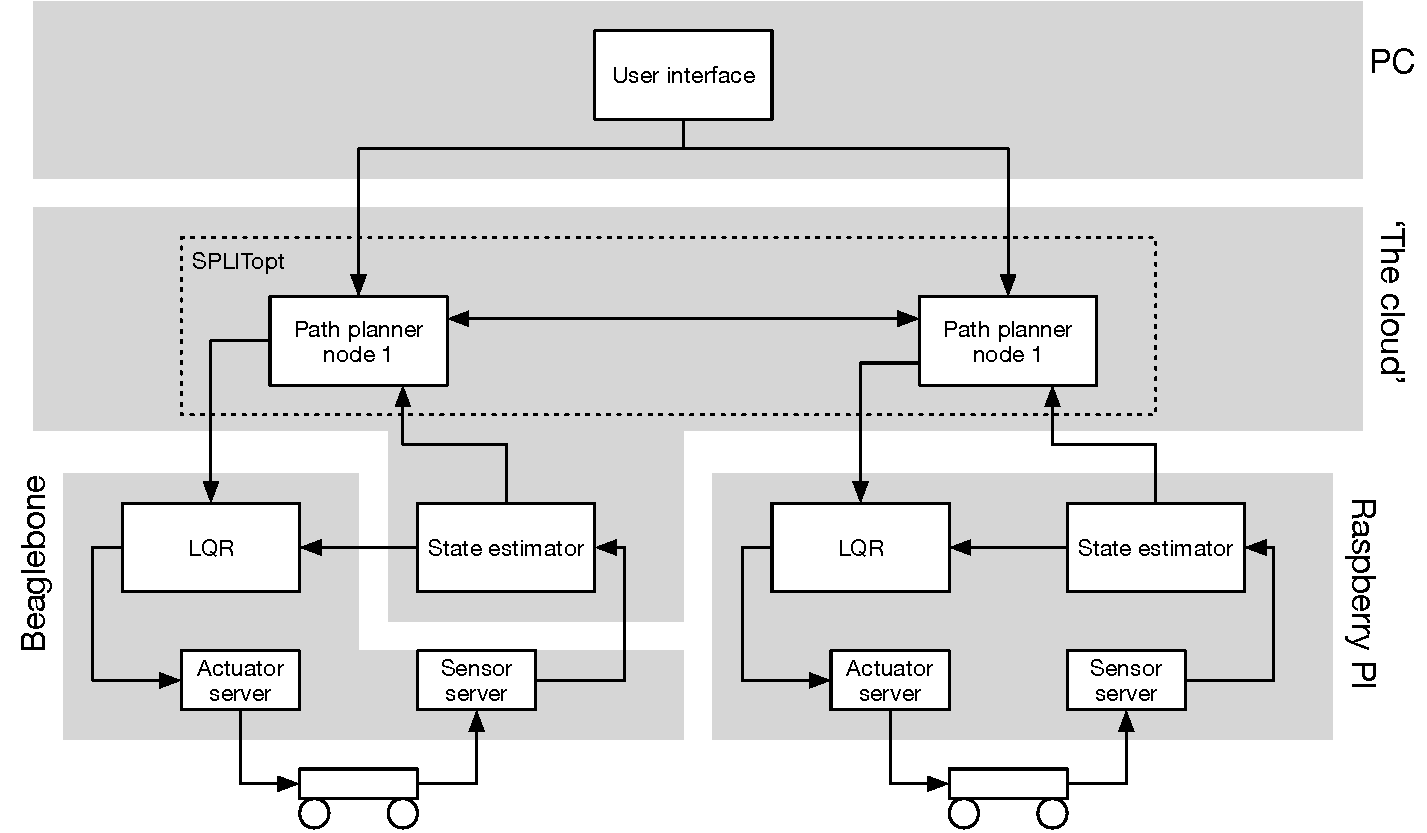
\includegraphics[width=0.9\textwidth]{split_use_case}


\section*{Components of SPLIT}
\begin{description}
  \item[OBN] This is openBuildNet with the global clock turned off, i.e., it runs only in its real-time mode rather than as a simulation.

  The `operating system' is made up of a set of \emph{nodes} that can send messages to defined channels, or register to receive messages from given channels. We have a variety of node types based on language: matlab, c, c++ and python. In each case, the user provides a list of channels that they want to register for, and a callback function for each message / trigger type.

  The network of nodes to be deployed is defined in a central descriptor file, which includes information about the hardware to which they're to be deployed, etc.

  Communications are handled by an existing IoT protocol (currently YARP).

  OBN has been thoroughly defined in a variety of live documents by Truong. The initial focus of the project has been on the simulation side, and this is where a lot of the complexity has arisen. A next step will be to decide how the platform would change in order to support real-time distributed computing.

  \item[SPLITmodeller] This is the module that converts from a high-level language description, does appropriate conversions (e.g., from m-files to c-files using matlab coder, or from an optimization description to a network of SPLITos nodes using SPLITopt, etc). 
\end{description}

We can think of each node in the network as a computational block with a clear trigger (sample time, arrival of data, etc), a computational task to execute (compute $Kx$, solve optimization problem, etc) and a set of outputs, which are written to a communication channel. The triggers and outputs are dealt with via OBN code, whereas the computational task must be defined by the user via SPLITmodeller.

SPLITmodeller has a number of different methods to define a computational task:
\begin{itemize}
  \item Directly as a c function, c++ function or python function. This is just included into the OBN wrapper code and compiled.
  \item m-function
  \begin{itemize}
    \item Converted to a c-function via matlab coder
    \item Embedded into a matlab node as a callback function
  \end{itemize}
  \item Local optimization problem. Converted to c-code via SPLITopt and wrapped in the OBN code
  \item Distributed optimization problem. 
\end{itemize}


  % \item[SPLITopt] This is what we call `SPLIT' today. This is a tool to translate from a high-level description of a parametric optimization problem to 

\newpage
\section*{SPLITopt}
This is the optimization package currently called `SPLIT'. Our goal is to generate fast code to solve distributed nonconvex parametric optimization problems described in a high-level language.

This part of the note is focused on how we should extend the current formulation to support nonlinear, possibly nonconvex and parametric distributed optimization problems.

Current formulation:
\begin{align*}
  \min\ &\frac{1}{2}x^\tp Qx + c^\tp x + \sum_i w_i h_i(T_ix + t_i)\\
  \text{s.t.}\ & Ax = b
\end{align*}
Where $h_i$ is a function with a well-defined (easy to solve) proximal operator.

This formulation supports the variables $c$ ,$t_i$ and $b$ being linearly parameterized. This is a major limitation because it effectively limits us to linear MPC formulations where only the state estimate varies (i.e., we can't handle systems that re-linearize online). Extending beyond this form will likely require a huge change (total re-write) in how these problems are parsed now, and a less significant change in how they are managed at solve-time.

A more general formulation would be:
\begin{align*}
  \min\ &f(x,\theta) + \sum_i w_i h_i(T_iy)\\
  \text{s.t.}\ & g(x,\theta) = 0\\
  &y = p(x,\theta)
  &Ax = b
\end{align*}
where each of the functions $f$, $p$ and $g$ are sums of functions of local variables:
\begin{align*}
f(x,\theta) = \sum_j f_j(x_j,\theta_j)
\end{align*}

If we have available the ability to generate online 


\newpage

\section*{What SPLIT is not / differentiation}
What are the unique features of SPLIT? How is it different from YALMIP, CVX, CVXPY, GPOPS, CASADI and ACADO?

The short answer : Distributed. Even a single device being controlled requires a base-station, network, high-frequency control loop and low-frequency optimization loop. SPLIT will be the platform to manage all this interconnection.

\begin{description}
  \item[Deployment] Since we want to do distributed optimization, managing the deployment across many   
  \item[Problem class] SPLIT is targeted at discrete-time optimization problems. We may one day be able to reuse the communication framework for translating from continuous to discrete time, but this is a relatively significant development. 
\end{description}

Summarizing the goals and limitations of existing tools:
\begin{itemize}
  \item YALMIP, CVX
  \begin{itemize}
    \item Pros : Excellent at simulation, and utilizing external tools
    \item Cons : Cannot deploy controllers. Centralized.
  \end{itemize}
  \item CVXPY
  \begin{itemize}
    \item Pros : Reaches an audience much larger than control.
    \item Cons : Can do distributed - but not for distributed control, only distributed optimization. Convex only (for now).
  \end{itemize}
  \item CaSaDi
  \begin{itemize}
    \item Pros : Provides nice algorithmic blocks to construct various optimization algorithms. A lot of this functionality could be gotten from sundials codes.
    \item Cons : PITA\footnote{Pain-in-the-ass} to install. Targeted at desktop systems (for now). Centralized.
  \end{itemize}
  \item ACADO
  \begin{itemize}
    \item Pros : Fast, well-developed solutions to continuous-time optimal control problems.
    \item Cons : Multiple-shooting only (not a huge limitation). `Only' generates optimization code, but doesn't provide the communication or supporting code. Centralized.
  \end{itemize}
\end{itemize}

\section*{Questions}

Do we want / not want the following?
\begin{itemize}
  \item Linking to external tools? Should we be YALMIP for \emph{deployment} of embedded optimization?
  \item How far do we want to go with communication and `linking' code? 
  \begin{itemize}
    \item Nothing: SPLIT just produces c-code for optimization
    \item Partial: SPLIT produces communication code for distributed optimization
    \item Total with partner: SPLIT allows for deployment of all the observers, low-level loops etc by using another existing tool (virtual arena? not sure there are many)
    \item Total: SPLIT is an end-to-end tool for the deployment of distributed controllers
  \end{itemize}
\end{itemize}

\section{Use Cases}
This section will outline a set of potential use cases for SPLIT.

\subsection{Embedded Optimization}
\begin{itemize}
  \item Deployment of Convex Optimizer for a Single Device
  \item Deployment of Convex Distributed Optimization Algorithms
\end{itemize}

\subsection{Solving / Analysis of Optimization Problems for Simulation (YALMIP replacement)}

\subsection{Deployment of Interfaces to Optimization Problems (Embedded YALMIP)}
YALMIP does a great job with the solution of optimization models from within MATLAB - there's no way that we should be re-developing this. However, there are a number of optimization tools (FORCES, ECOS, CPLEX, etc) that would be nice to utilize in an embedded environment from the same interface as if we were using it in MATLAB.

\subsection{Development of Novel Optimization Methods}
Ideally, we would be able to maximize re-use of the key pieces of an optimization modeling and deployment tool to rapidly develop novel algorithms. This is the direction that CaSaDi is going in for continuous, non-linear optimization problems by providing the integration and sensitivity components. It would be very nice to do this also for distributed optimization problems arising from discrete-time systems.

Achieving this requires a number of different standard components:
\begin{itemize}
  \item Modeling : Parsing high-level expressions into a standard form
  \item Problem formulation : Conversion from standard form to the structure required for the optimization method (i.e., moving to an augmented Lagrangian, etc)
  \item Linear algebra : Auto-customized linear algebra routines where useful
  \item Management of data, etc
  \item Communication modules
\end{itemize}

\subsection{Non-convex}
There's not much difference between convex and non-convex solvers. The key difference is that the data matrices are changing dynamically either per iteration, or per solve based on a linearization. To solve non-convex problems, we will need:
\begin{itemize}
  \item Auto-generated / tuned fast linearization routines
  \item asdf
\end{itemize}


\section{Tying it Together : The Communication and Connection Modules}



\section{Timeline}




\end{document}